\documentclass[a4paper,12pt]{article}
\usepackage[utf8]{inputenc}
\usepackage[russian]{babel} 
\usepackage{graphicx} 
\usepackage{amsmath}
\usepackage{amssymb}
\usepackage{float}
\usepackage[colorlinks=true, linkcolor=blue]{hyperref}
\usepackage{enumitem}

\renewcommand{\floatpagefraction}{0.99}
\renewcommand{\topfraction}{0.99}      


%\title{Лабораторная работа №4.1}
\title{ Задача "Рёв Быка".}


\author{Батанин Артём Александрович}
\date{\today}


\begin{document}

\maketitle

\newpage
\tableofcontents    
\newpage            

\section{Вращение пластины относительно своей оси}
В момент начала движения пластина располагалась случайным образом относительно направления движения. Из-за некоторого ненулевого угла между набегающим потоком воздуха и плоскостью пластины (далее - угла атаки) возникает момент силы из за неравномерного действия силы сопротивления воздуха на пластину, который начинает раскручивать пластину вдоль своей оси \ref{fig:potok}.

\begin{figure}[h!]
\centering
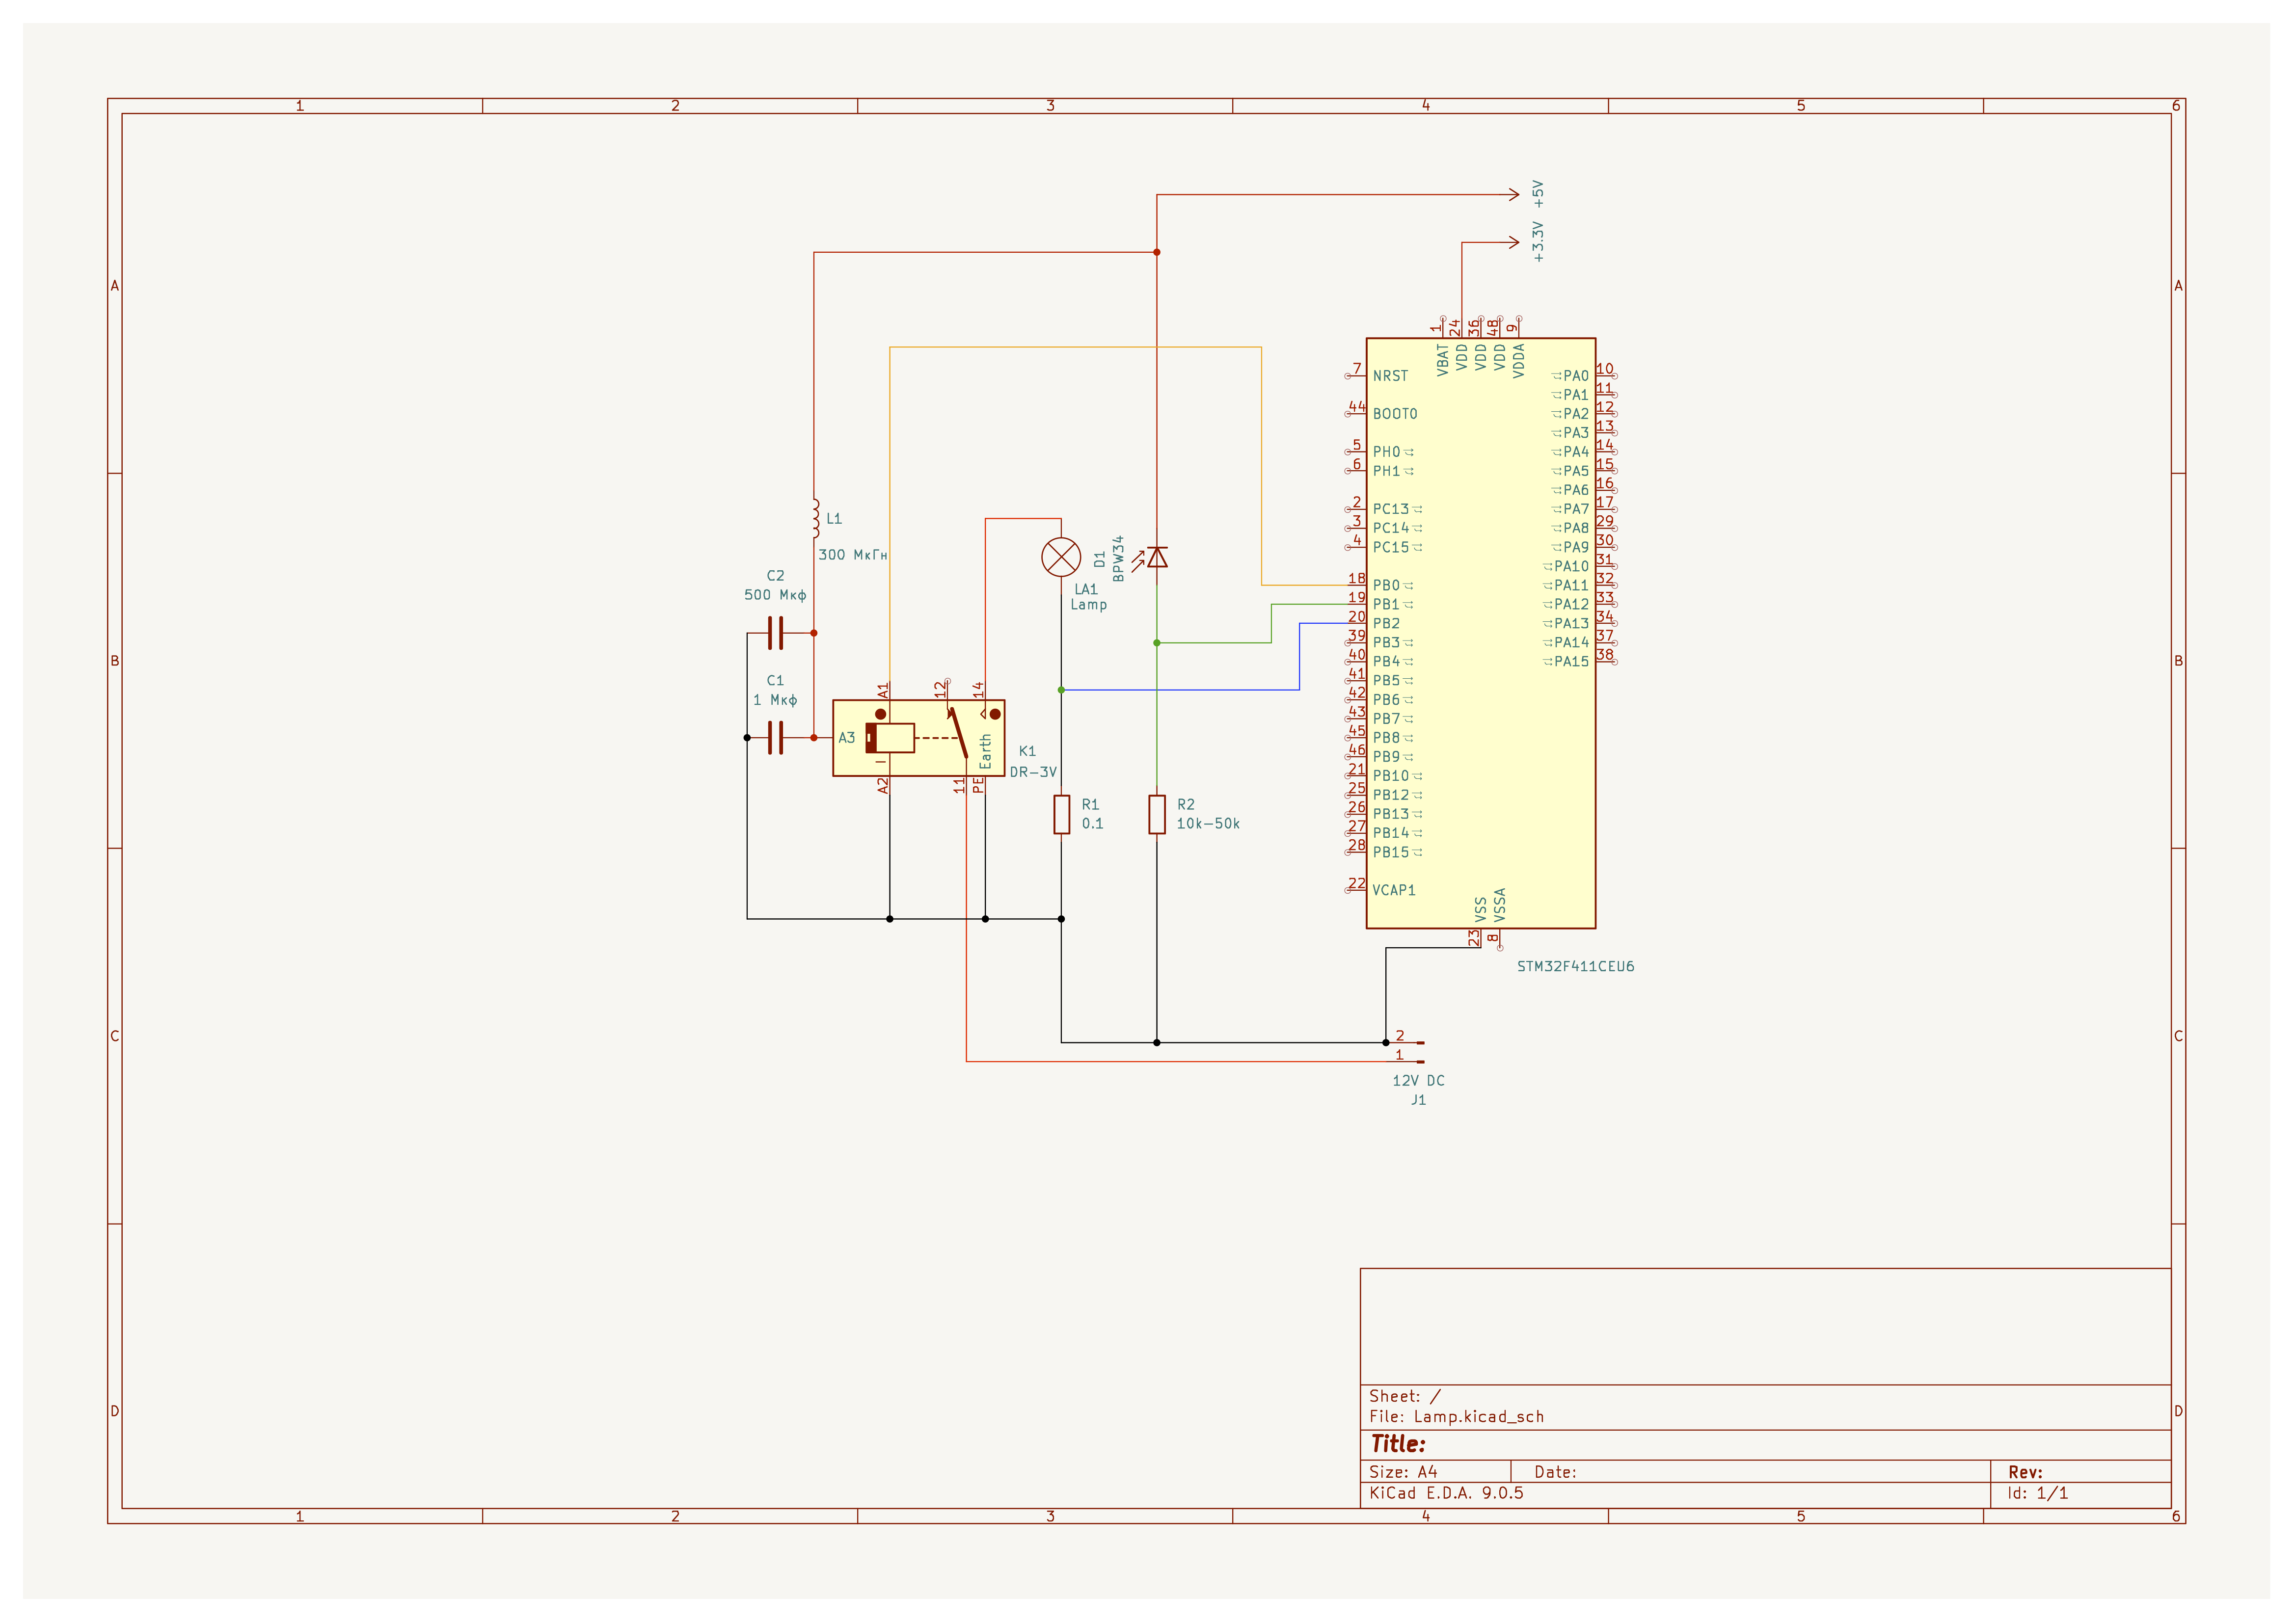
\includegraphics[width=1\linewidth]{Schema.png}
\caption{Обтекание пластины воздушным потоком}
\label{fig:potok}
\end{figure}

Из модели обтекания воздухом видно, что наибольшее давление (а следовательно и сила) действует на верхнюю треть пластины. Т.к силы в верхней и нижней части пластины создают разные моменты - пластина начинает раскручиваться. Возникает самоподдерживающееся вращение пластины (авторотация).




\section{Подъёмная сила}
Из-за вращения верхний и нижний конец пластины имеют разные скорости.
\begin{figure}[h!]
\centering
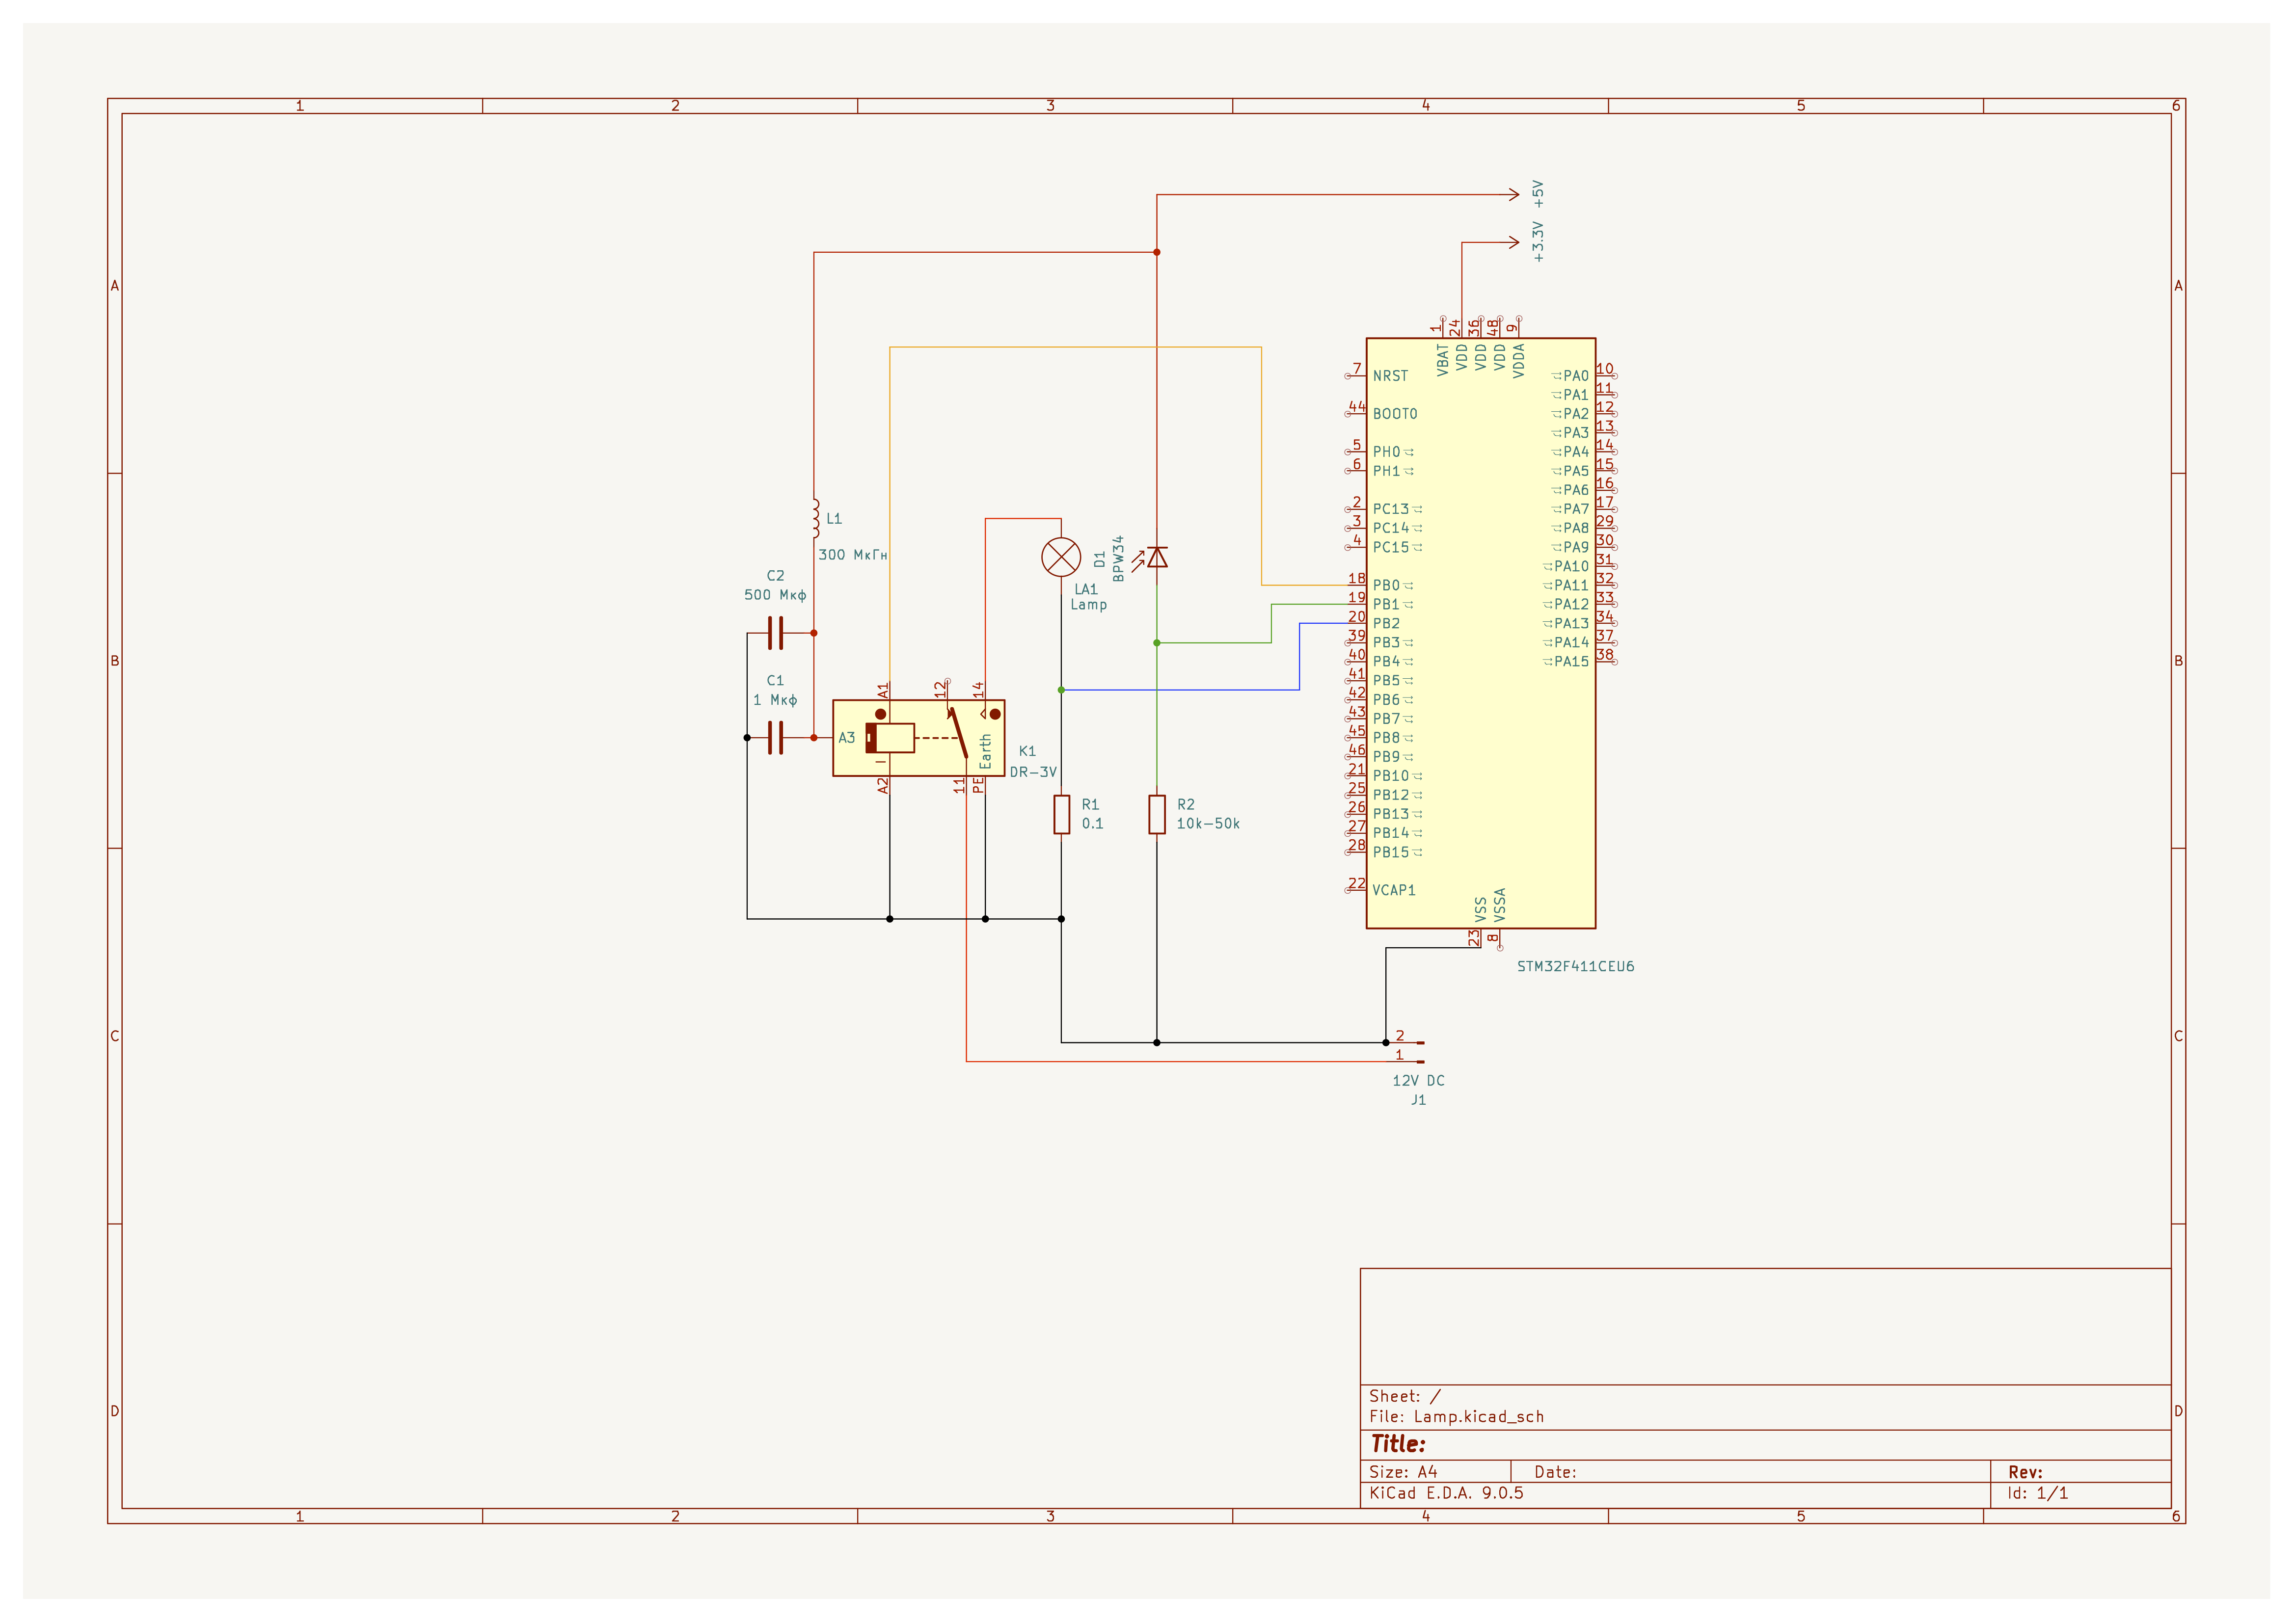
\includegraphics[width=1\linewidth]{Schema.png}
\caption{Возникновение подтёмной силы}
\label{fig:speeds}
\end{figure}
 Согласно закону Бернулли ($\frac{\rho \cdot v^2}{2} +p = const$) давление, действующее на половину пластины, движущуюся сонаправлено воздуху будет выше чем давление, действующую на вторую половину. Из разницы давлений возникает подъёмная сила, действующая перпендикулярно потоку воздуха (относительно пластины) и оси вращения пластины (Эффект Магнуса).

$F_{\mu} = 1/2 \cdot C_M \cdot \rho \cdot V^2 \cdot S$ - Формула для рассчёта подьёмной силы за счёт эффекта магнуса, где $C_M$ - коэффициент силы Магнуса, зависящий от геометрии дощечки и характера её вращения. (Определяется эмпирически)


\section{Верхняя и нижняя фазы}
Вращаясь, пластина закручивает верёвку, на которую она закреплена. Верёвка начинает создавать момент вращения, направленный противоположно моменту, создаваемому в ходе авторотации. Когда моменты становятся равны, пластина перестаёт вращаться, после чего эффект авторотации начинает раскручивать пластину в противоположную сторону. Верёвка раскручивается и вновь закручивается в другую сторону - вращение периодически повторяется. 
Из-за того, что пластина вращается то в одну, то в другую сторону, эффект Магнуса действует в разные стороны - вверх или вниз.
\subsection{Верхняя фаза}

\begin{figure}[h!]
\centering
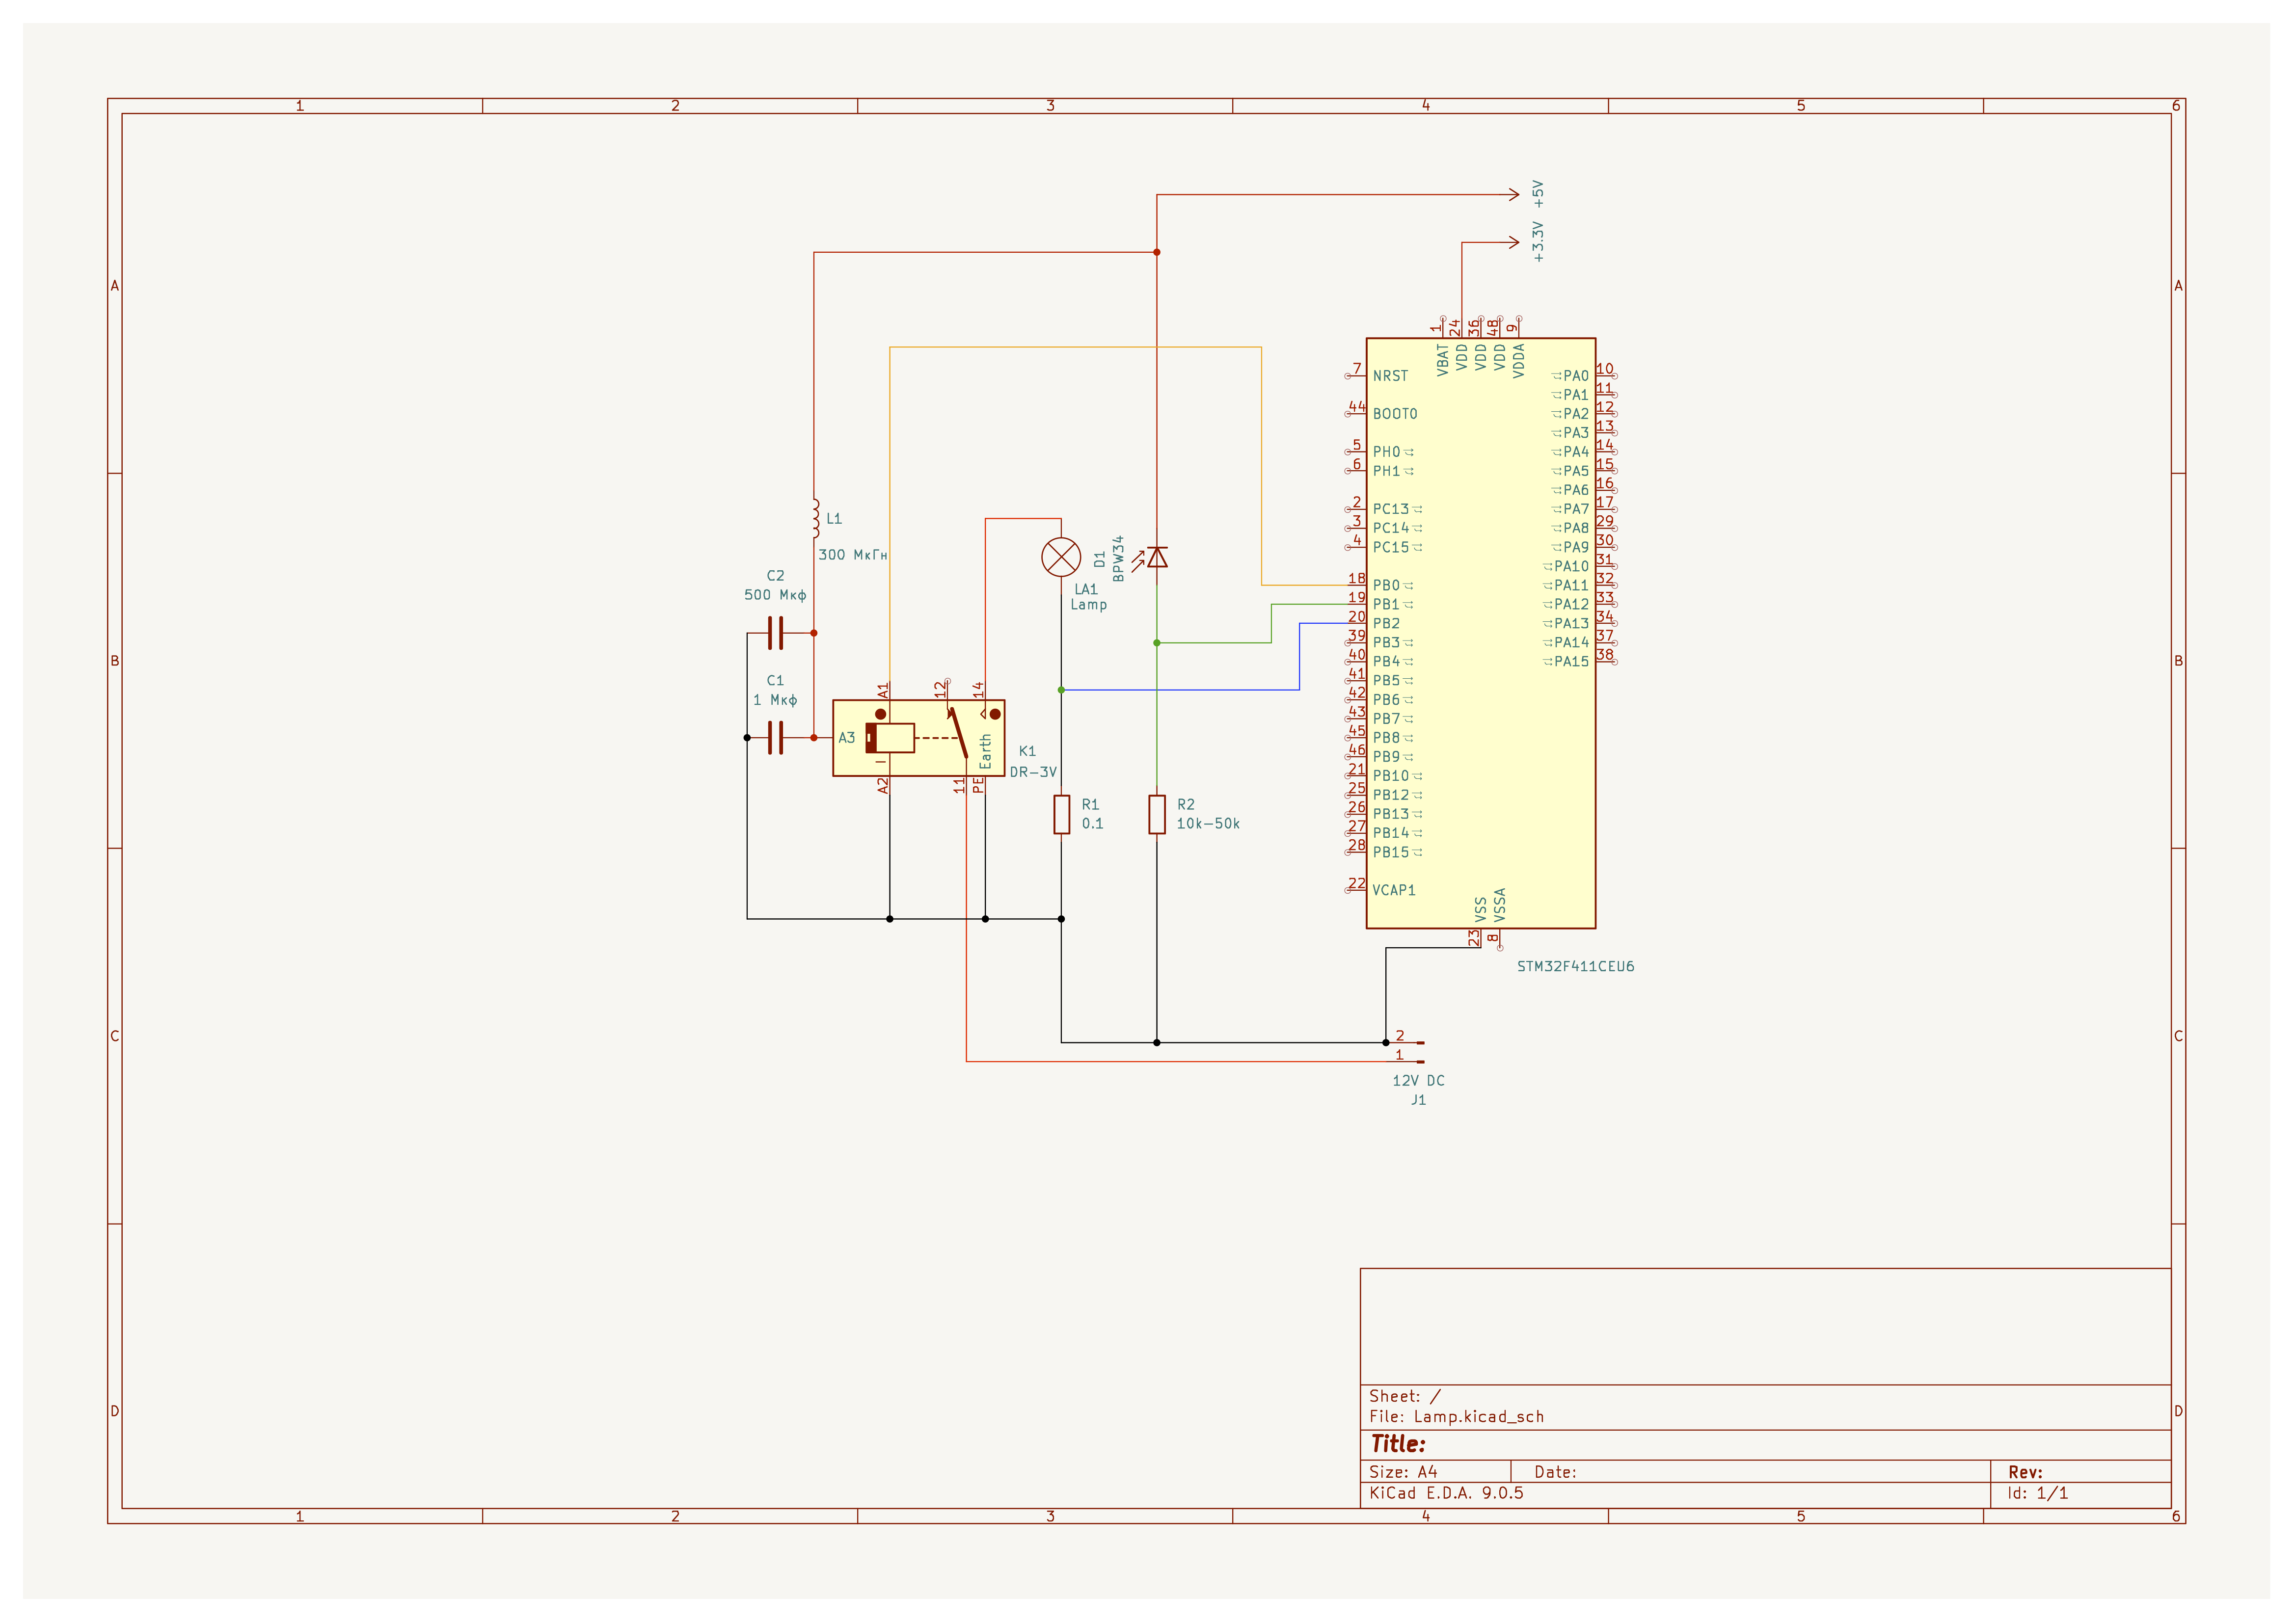
\includegraphics[width=1\linewidth]{Schema.png}
\caption{Верхняя фаза вращения}
\label{fig:up}
\end{figure}

Верхняя фаза вращения - фаза, где вращение пластины относительно своей оси направлено таким образом, что верхний конец пластины движется сонаправленно с собственным движением пластины (следовательно достигается наибольшая скорость верхнего конца  относительно воздуха), а нижняя противоположно направленно. Из-за разницы давлений подъёмная сила действует вверх. выражение для угла  $\alpha$: 

\begin{equation} 
    \begin{gathered}
	\tan(\alpha )= \frac{F_{\mu} - mg}{m \cdot v^2 / R \cdot \cos{\alpha}}\\
	\tan(\alpha )= \frac{ (F_{\mu} - mg) \cdot R \cdot \cos{\alpha}}{m \cdot v^2}\\
	\frac{\sin(\alpha) }{\cos^2(\alpha) }= \frac{ (F_{\mu} - mg) \cdot R }{m \cdot v^2}\\
	\frac{\sin(\alpha) }{1-\sin^2(\alpha) }= \frac{ (F_{\mu} - mg) \cdot R}{m \cdot v^2} \\
	\frac{ (1-\sin^2\alpha) \cdot (F_{\mu} - mg) \cdot R}{m \cdot v^2} - \sin(\alpha) = 0\\
	\alpha = \arcsin(\frac{\sqrt{1+4k^2} - 1}{2k}) \\
		    \end{gathered}
    \end{equation}
 где $k =  \frac{ (F_{\mu} - mg) \cdot R}{m \cdot v^2} $





\subsection{Нижняя фаза}
Нижняя фаза описывается аналогично верхней. Выражение для угла:
$\alpha = - \arcsin(\frac{\sqrt{1+4k^2} - 1}{2k}) $
 где $k =  \frac{ (F_{\mu} + mg) \cdot R}{m \cdot v^2} $

\begin{figure}[h!]
\centering
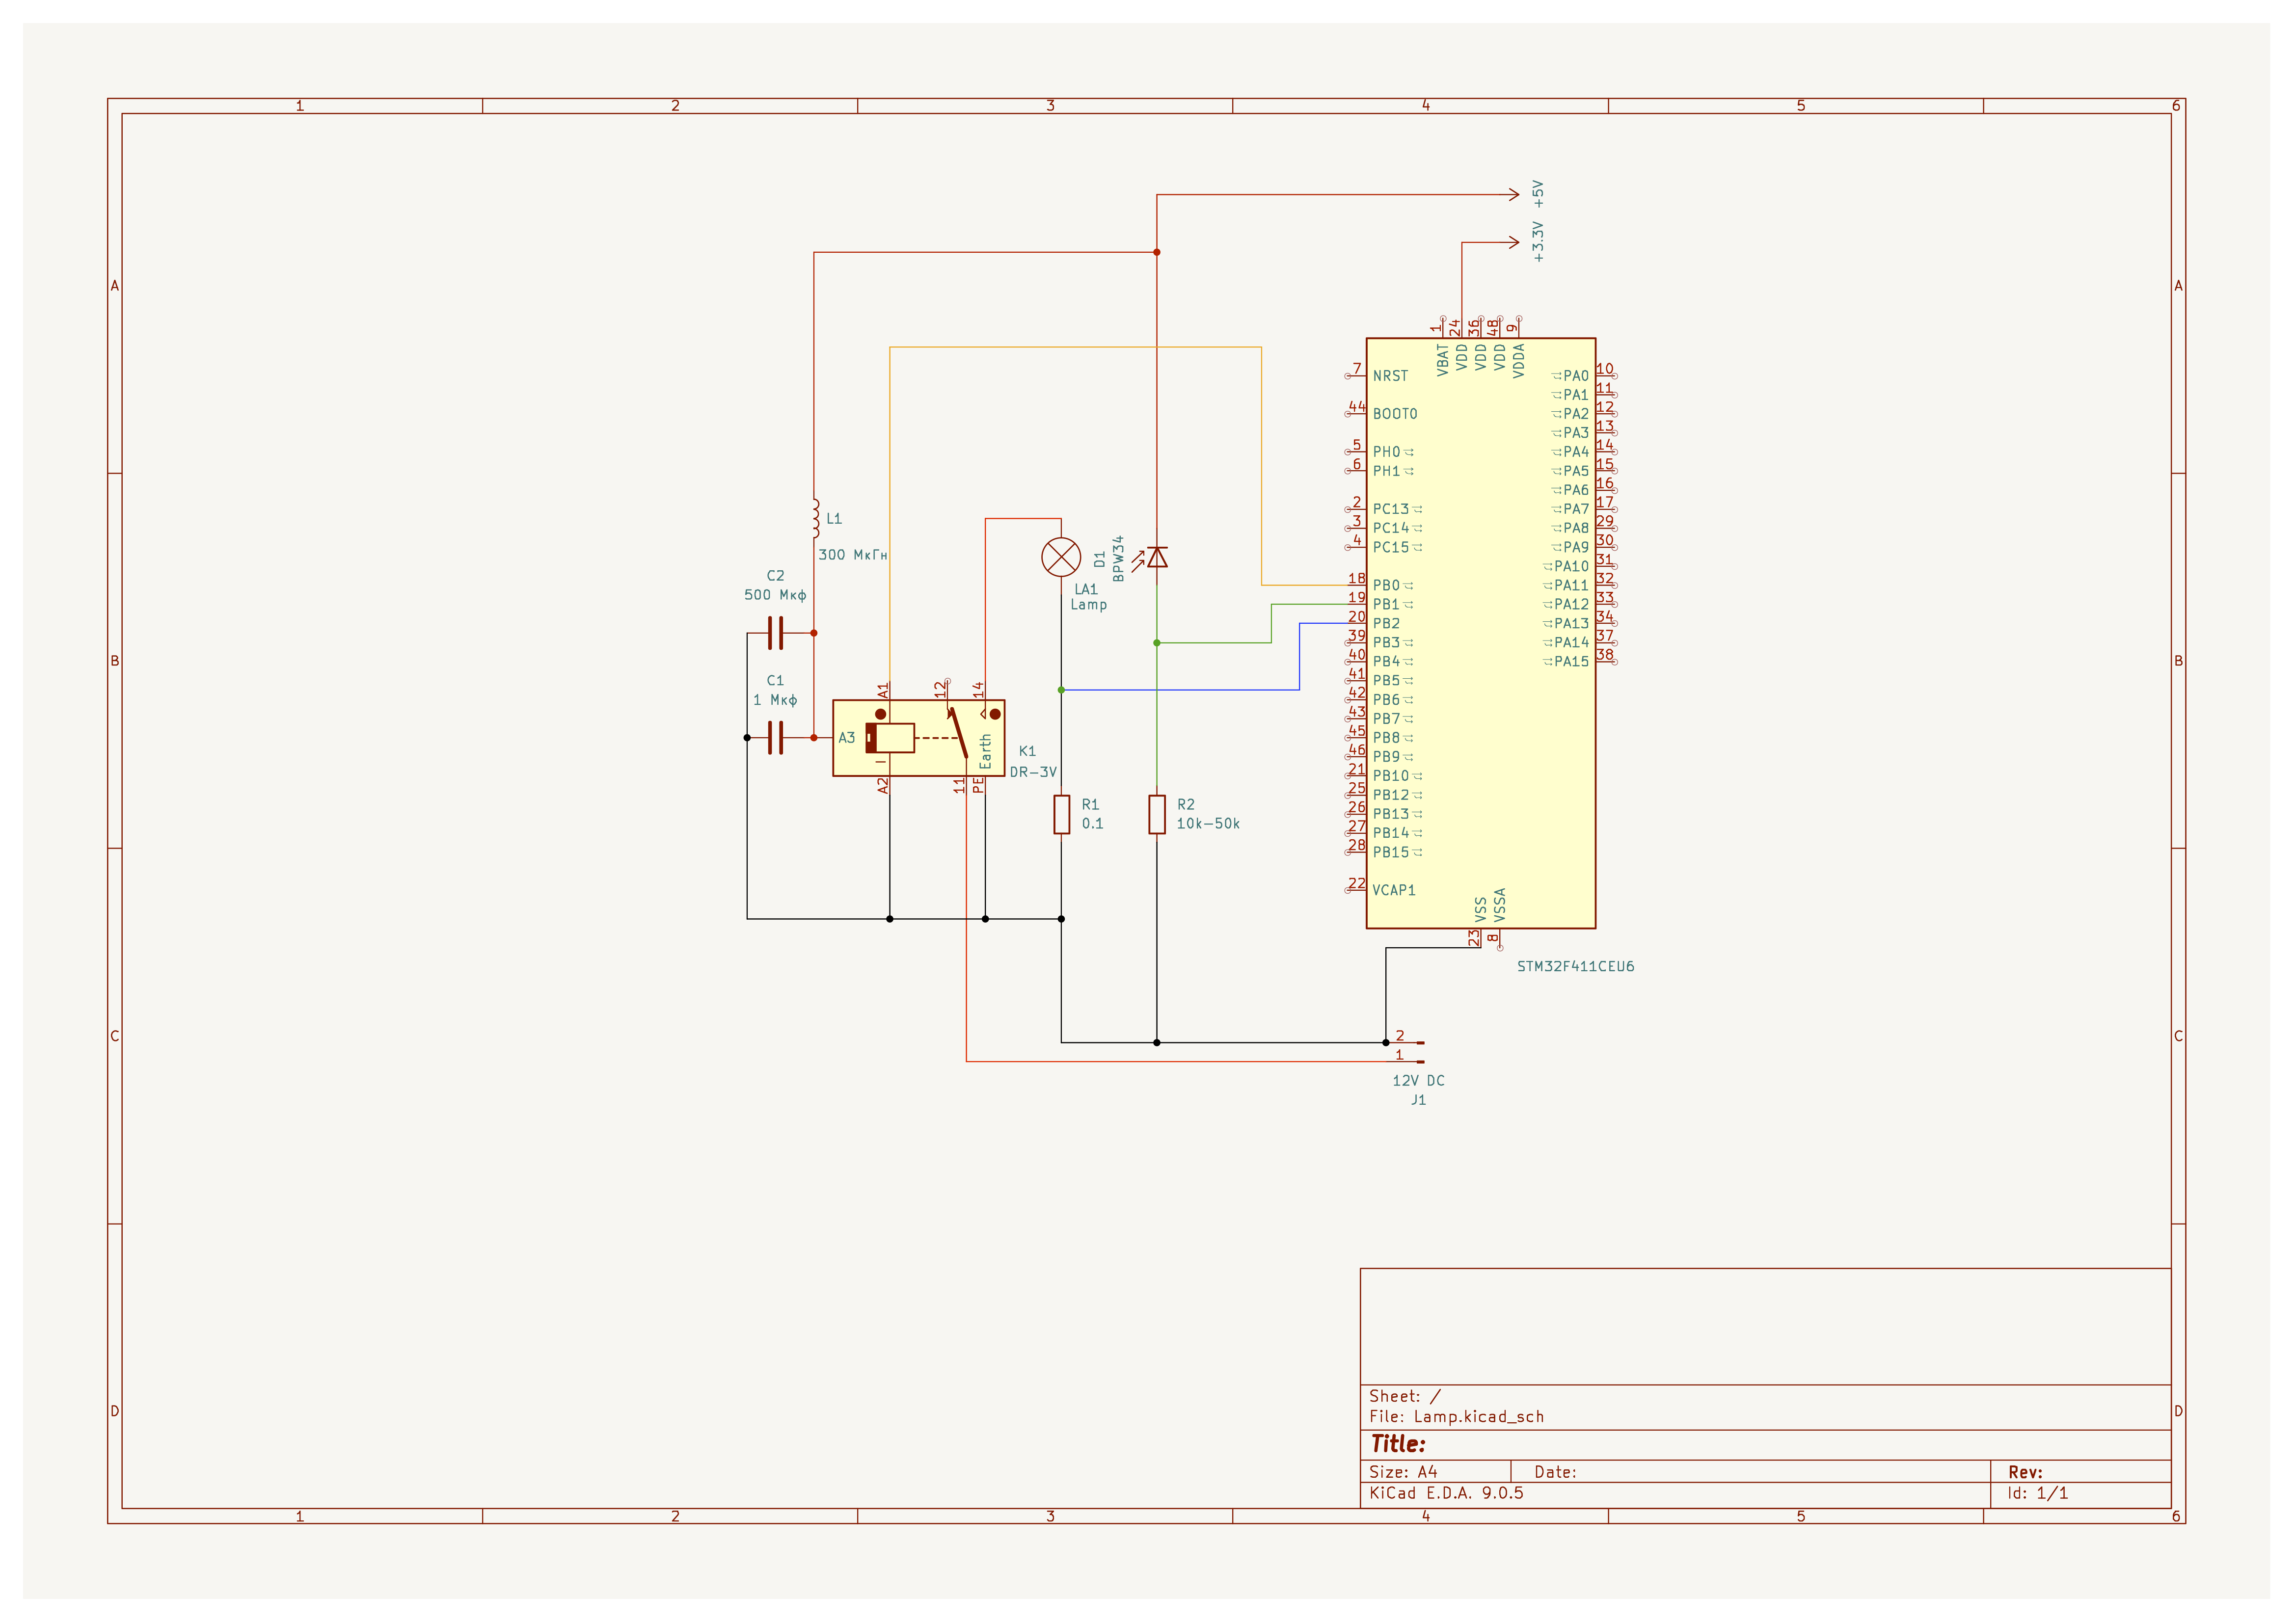
\includegraphics[width=1\linewidth]{Schema.png}
\caption{Нижняя фаза вращения}
\label{fig:up}
\end{figure}




\section{Появление звука}
Из-за вращения дощечки образуются области повышенного и пониженного давления, которые сменяют друг друга в пространстве. Эти колебания плотности - и есть звуковая волна. чем чащу вращается дощечка тем с более высокой частотой издаётся гул.



\section{Примечание}
На \autoref{fig:potok} изображено решение уравнений Максвелла для проводника в поток э-м поле. Для скоростей движения значительно меньше скорости звука, уравнения Максвелла в таких случаях эквивалентны уравнениям гидродинамики.

\end{document}